%!TEX root = ../thesis.tex

%%%%%%%%%%%%%%%%%%%%%%
%      Samples       %
%%%%%%%%%%%%%%%%%%%%%%
\message{^^J ^^J SAMPLES ^^J ^^J} % print to log
\newchap{Data sets \& Simulated Samples} \label{sec:samples}

This chapter will discuss in more detail the data sets of $\Pp\Pp$ collision events used, as well as the samples of simulated background events.


%%%%%%%%%%%%
%   DATA   %
%%%%%%%%%%%%
\section{Data sets} \label{sec:data}

The total data set recorded between 2016 and 2018 corresponds to an integrated luminosity of approximately 138\fbinv at $\sqrt{s}=13\TeV$. The run ranges and integrated luminosity per year are listed in Table~\ref{tab:data_runnumbers}.

% TABLE: data
%!TEX root = ../thesis.tex

\begin{table}[h!]
\vspace{-1mm}
\centering
\caption{LHC run number ranges and corresponding integrated luminosity $L$ recorded by CMS and certified for physics analysis.}
\label{tab:data_runnumbers}
\begin{tabular}{lr}
  \hline
  Run number range & $L$ [{\fbinv}] \\
  \hline
  272007--284044 & 36.3 \\
  297020--306462 & 41.5 \\
  315252--325175 & 59.7 \\
  \hline
\end{tabular}
\vspace{-1mm}
\end{table}



% FIGURE: Simulation
%!TEX root = ../thesis.tex

% FIGURE: event generation
% https://www.zora.uzh.ch/id/eprint/32078/41/Gleisberg_JHEP_AM_2009_V.pdf
\begin{figure*}[bp]
  %\vspace{-2mm}
  \centering
  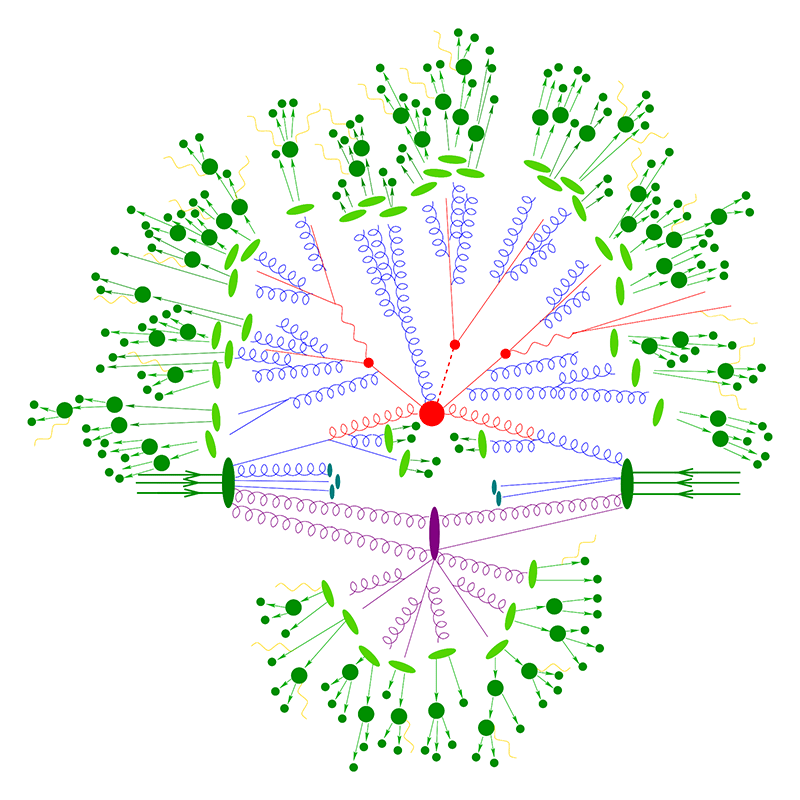
\includegraphics[width=0.82\textwidth]{fig/samples/simulation_event_generation.png}
  \vspace{-4mm}
  \caption{
Schematic diagram explaining event generation of two colliding protons.
Retrieved from~\cite{event_generation_fig}.
  } \label{fig:event_generation}
  \vspace{-8mm}
\end{figure*}


%%%%%%%%%%%%%%%%%%
%   SIMULATION   %
%%%%%%%%%%%%%%%%%%
\section{Event simulation} \label{sec:simulation}

The \PYTHIA parameters affecting the description of the underlying event are set to the {CUETP8M1} ({CP5}) tune for all 2016 (2017 and 2018) samples~\cite{TuneCUETP8M1,TuneCP}, except for the 2016 $\ttbar$ sample, for which {CUETP8M2T4}~\cite{TuneCUETP8M2T4} is used.
The interaction with the CMS detector is simulated by \GEANTfour~\cite{GEANT4}.
Pileup is generated with \PYTHIA.
Event generation is described in more detail in Refs.~\cite[p.~717]{PDG_2022}, \cite{event_generation} and~\cite{Pythia6_manual}.


%%%%%%%%%%%%%%%%%%
%   BACKGROUND   %
%%%%%%%%%%%%%%%%%%
\section{Backgrounds} \label{sec:background}

% TABLE: backgrounds
%!TEX root = ../thesis.tex

\begin{table}[pt]
\vspace{-10mm}
\caption{Summary of simulated SM backgrounds, including generator(s) and cross sections (for 2017 \& 2018 samples with the CP5 tune). Drell-Yan and $\Wjets$ samples with ``$+\,\text{$n$ jets}$'' refer to a fixed number of partons, $n$, at the level of the hard process in \MADGRAPH.}
\label{tab:samples_background}
\centerline{
\begin{tabular}{lll}
  \hline
  Process & Generators & Cross section $\sigma$ [pb] \\
  \hline
  \tabsubtitle{Drell-Yan, $\Zg\to\LL$, LO} \\
  \;$+\,\text{jets}$, $10<\mll<50\GeV$ & \MADGRAPH, \PYTHIA  & 15810.0 (LO), 18610.0 (NLO) \\
  %\;$(\Zg\to\LL)+\text{jets}$, $\mll\in[10,50[\GeV$ & \MADGRAPH, \PYTHIA  & 15810.0 (LO), 18610.0 (NLO) \\
  \;$+\,\text{jets}$, $\mll>50\GeV$    & \MADGRAPH, \PYTHIA  & 5343.0 (LO), 6077.2 (NNLO) \\ % 3*2025.74
  \;$+\,\text{1 jets}$, $\mll>50\GeV$    & \MADGRAPH, \PYTHIA  & 877.8 (LO) \\
  \;$+\,\text{2 jets}$, $\mll>50\GeV$    & \MADGRAPH, \PYTHIA  & 304.4 (LO) \\
  \;$+\,\text{3 jets}$, $\mll>50\GeV$    & \MADGRAPH, \PYTHIA  & 111.5 (LO) \\
  \;$+\,\text{4 jets}$, $\mll>50\GeV$    & \MADGRAPH, \PYTHIA  & 44.05 (LO) \\
  
  \tabsubtitle{Drell-Yan, $\Zg\to\LL$, NLO} \\
  \;$+\,\text{jets}$, $\mll\in[100,200[\GeV$     & \aMCATNLO, \PYTHIA   & 247.8 (NLO)    \\
  \;$+\,\text{jets}$, $\mll\in[200,400[\GeV$     & \aMCATNLO, \PYTHIA   & 8.502 (NLO)    \\
  \;$+\,\text{jets}$, $\mll\in[400,500[\GeV$     & \aMCATNLO, \PYTHIA   & 0.4514 (NLO)   \\
  \;$+\,\text{jets}$, $\mll\in[500,700[\GeV$     & \aMCATNLO, \PYTHIA   & 0.2558 (NLO)   \\
  \;$+\,\text{jets}$, $\mll\in[700,800[\GeV$     & \aMCATNLO, \PYTHIA   & 0.04023 (NLO)  \\
  \;$+\,\text{jets}$, $\mll\in[800,1000[\GeV$    & \aMCATNLO, \PYTHIA   & 0.03406 (NLO)  \\
  \;$+\,\text{jets}$, $\mll\in[1000,1500[\GeV$   & \aMCATNLO, \PYTHIA   & 0.01828 (NLO)  \\
  \;$+\,\text{jets}$, $\mll\in[1500,2000[\GeV$   & \aMCATNLO, \PYTHIA   & 0.002367 (NLO) \\
  \;$+\,\text{jets}$, $\mll\in[2000,3000[\GeV$   & \aMCATNLO, \PYTHIA   & $5.409\times10^{-4}$ (NLO) \\
  \;$+\,\text{jets}$, $\mll\in[3000,\infty[\GeV$ & \aMCATNLO, \PYTHIA   & $3.048\times10^{-5}$ (NLO) \\
  
  \tabsubtitle{\Wjets, $\PW\to\ell\nu$} \\
  \;$+\,\text{jets}$    & \MADGRAPH, \PYTHIA  & 52940.0 (LO), 61526.7 (NLO) \\
  \;$+\,\text{1 jets}$  & \MADGRAPH, \PYTHIA  & 8104.0 (LO) \\
  \;$+\,\text{2 jets}$  & \MADGRAPH, \PYTHIA  & 2793.0 (LO) \\
  \;$+\,\text{3 jets}$  & \MADGRAPH, \PYTHIA  & 992.5 (LO) \\
  \;$+\,\text{4 jets}$  & \MADGRAPH, \PYTHIA  & 544.3 (LO) \\
  
  \tabsubtitle{$\ttbar+\text{jets}$} &       & 833.9 (NNLO) \\
  % https://twiki.cern.ch/twiki/bin/view/LHCPhysics/TtbarNNLO
  \;Fully leptonic      & \POWHEG, \PYTHIA   & 88.29 (NNLO), $\BF=10.6\%$ \\
  \;Semi-leptonic       & \POWHEG, \PYTHIA   & 365.35 (NNLO), $\BF=43.9\%$ \\
  \;Fully Hadronic      & \POWHEG, \PYTHIA   & 377.96 (NNLO), $\BF=45.4\%$ \\
  
  \tabsubtitle{Single top} \\
  % https://twiki.cern.ch/twiki/bin/view/LHCPhysics/SingleTopRefXsec
  \;$\PQt+\PW^-$                & \POWHEG, \PYTHIA  &  35.85 (NNLO) \\
  \;$\PAQt+\PW^+$               & \POWHEG, \PYTHIA  &  35.85 (NNLO) \\
  \;Single $\PQt$, $t$ channel  & \POWHEG, \PYTHIA  & 136.02 (NNLO) \\
  \;Single $\PAQt$, $t$ channel & \POWHEG, \PYTHIA  &  80.95 (NNLO) \\
  
  % https://cms-gen-dev.cern.ch/xsdb/?columns=67108863&currentPage=0&ordDirection=1&ordFieldName=process_name&pageSize=50&searchQuery=process_name%3D%5E%5BWZ%5D%5BWZ%5D_Tune%2A
  \tabsubtitle{Diboson} \\
  \;WW & \PYTHIA  & 75.88 (LO) \\ % TODO: REALLY LO !?!?!?!?!?!?!?
  \;WZ & \PYTHIA  & 27.60 (LO) \\
  \;ZZ & \PYTHIA  & 12.14 (LO) \\
  
  \hline
\end{tabular}}
\vspace{-1mm}
\end{table}


% SAMPLES
\subsection{Simulated backgrounds} \label{sec:background_simulation}

All the simulated background samples used in this thesis are listed in Table~\ref{tab:samples_background}.
The $\Wjets$ and $\Zjets$ processes are generated with \MADGRAPH~\cite{MadGraph} at LO precision.
The MLM jet matching and merging scheme~\cite{MLM} is used to match partons between \MADGRAPH and \PYTHIA and prevent overcounting.
The $\Zjets$ samples generated at NLO by \MGvATNLO~\cite{aMCatNLO}. 
The production of $\ttbar$ and singly produced top quarks is simulated with the \POWHEG~\cite{POWHEG0,POWHEG1,POWHEG2} 2.0 and 1.0 generators, respectively, at NLO precision~\cite{POWHEG_TT,POWHEG_TT2,POWHEG_ST_st,POWHEG_ST_tW}.
Diboson production is generated at LO with \PYTHIA 8~\cite{Pythia8,Pythia8_2015}.
The NNPDF3.0 PDF sets~\cite{NNPDF30} are used for 2016. The NNPDF3.1 PDF~\cite{NNPDF31} sets are used for 2017 and 2018 samples.

% CROSS SECTIONS
\subsection{Cross sections} \label{sec:background_xsecs}
% https://twiki.cern.ch/twiki/bin/view/LHCPhysics/TtbarNNLO
% https://twiki.cern.ch/twiki/bin/view/LHCPhysics/SingleTopRefXsec?rev=33#Single_top_Wt_channel_cross_sect
% https://twiki.cern.ch/twiki/bin/view/CMS/SummaryTable1G25ns#TTbar
Table~\ref{tab:samples_background} also lists the theoretical cross sections $\sigma$ for each sample.
The events are weighted by
\begin{equation} \label{eq:LsigmaN}
  Z = \frac{L\sigma}{N_\text{tot}},
\end{equation}
or with generator weight $w_\text{gen}$,
\begin{equation}
  Z = \frac{L\sigma}{\sum w_\text{gen}} w_\text{gen}.
\end{equation}
The LO cross sections of the $\Zjets$ and $\Wjets$ samples in Table~\ref{tab:samples_background} are computed with \MADGRAPH.
The $\Zjets$ cross section is computed with \FEWZ~\cite{FEWZ} program at NNLO in perturbative QCD, and with NLO electroweak corrections.
The $\ttbar+\text{jets}$ cross section was computed with the {\Toppp}v2.0 program~\cite{sigma_TT,sigma_TT_TWiki} at NNLO and at next-to-next-to-leading logarithmic (NNLL) accuracy.
The $\Wjets$ production is normalized with cross sections computed at NLO accuracy.
